\usepackage{stmaryrd}This lab was an introduction to the usage of a Linux (Ubuntu distro) VM on a host machine, and the usage of OpenSSL to
encrypt and decrypt data using the (outdated) DES algorithm and AES256 symmetric encryption algorithm.
Additionally, this lab looked at RSA private keys used in asymmetric encryption, and how to generate and gather
public and private keys, alongside message digests.

\section{Version checking and ciphers}\label{sec:version}
To check the installed version of OpenSSL, the command "openssl version" can be used.
The provided virtual machine from \href{https://moodle.bcu.ac.uk/mod/url/view.php?id=7914090}{the CMP5329 Moodle page}
uses OpenSSL version 1.1.1f, dated 31st March 2020.\footnote{This is a heavily outdated version of OpenSSL,
    however I have continued to use it due to it being part of the module-provided resources.}

\begin{figure}[H]
    \centering
    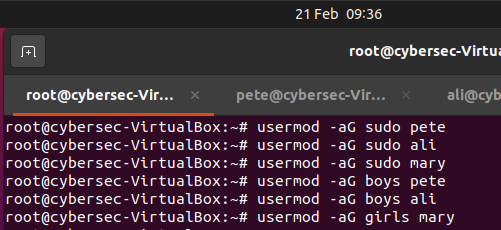
\includegraphics[width=.9\linewidth]{lab1/2}
    \caption{Getting the OpenSSL version}
    \label{fig:version}
\end{figure}

The list of OpenSSL ciphers can be viewed by executing the "openssl ciphers" command.

\begin{figure}[H]
    \centering
    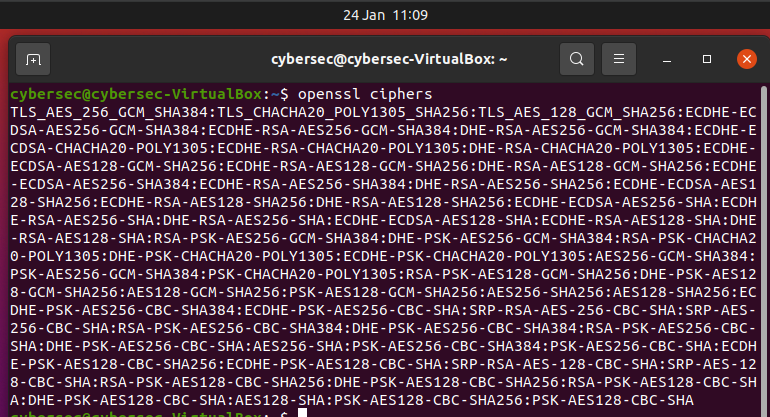
\includegraphics[width=.9\linewidth]{lab1/3}
    \caption{Getting the OpenSSL ciphers}
    \label{fig:ciphers}
\end{figure}

\section{Symmetric encryption}\label{sec:symmEncrypt}
Symmetric cryptography refers to the process of transferring data that has been encrypted by a single key.
Both the sender and receiver of this data use the same key to encrypt and decrypt the data.
Symmetric encryption does not allow for non-repudiation, as it cannot necessarily be proven that data came
from one sender and not someone else with the key, as there is no attached signature to prove the sender's
identity.

\subsection{DES symmetric encryption}\label{subsec:des}
OpenSSL can be used to encrypt plaintext into unreadable text known as ciphertext.
Many algorithms exist to generate ciphertext, but for this example, the Data Encryption Standard (DES)
symmetric encryption algorithm will be used.
This is performed using the command \newline"openssl enc -des -k secretkey -a".
\footnote{"echo a secret message | " passes the phrase "a secret message" as the text to be encrypted.}
This command can be broken down into:

\begin{itemize}
    \item enc - Encode
    \item -des - Using the DES algorithm
    \item -k secretkey - Using the key "secretkey"
    \item -a - Writes the ciphertext in base64, allowing it to be properly displayed.
               If this flag isn't used, the text will not be legible, showing question mark symbols instead.
\end{itemize}

\begin{figure}[H]
    \centering
    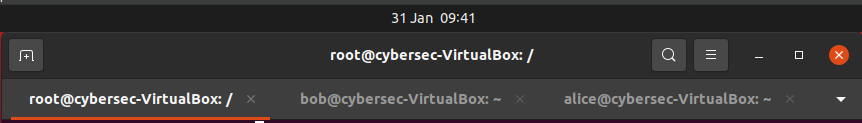
\includegraphics[width=.9\linewidth]{lab1/4}
    \caption{Converting "a secret message" to ciphertext using DES with key "secretkey".}
    \label{fig:DESEncrypt}
\end{figure}

This ciphertext can then be decoded if you know the key it was encoded with.

\begin{figure}[H]
    \centering
    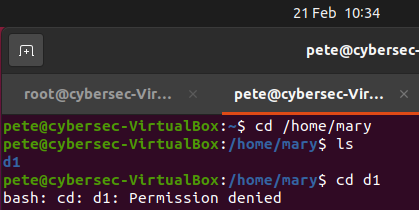
\includegraphics[width=.9\linewidth]{lab1/5}
    \caption{Decoding the ciphertext back to its original form using the key "secretkey".}
    \label{fig:DESDecrypt}
\end{figure}

This command is the same as in Figure~\ref{fig:DESEncrypt}, with two alterations:
\begin{itemize}
    \item The ciphertext is passed to OpenSSL rather than the plaintext, as we typically wouldn't know
          the original plaintext in this scenario, which is what we are aiming to achieve by decrypting it.
    \item -d - Indicates that the text should be decrypted rather than encrypted.
\end{itemize}\newline

\pagebreak

\subsection{AES256 symmetric encryption and decryption}\label{subsec:aes256}
The DES algorithm is considered weak to today's standards due to how simple it is to
brute-force using today's processing power.
Because of this, newer algorithms were developed, with one of these being AES\@.
AES256 refers to the key size, which is 256 bits for this variant, though you can use key sizes of
128 or 192 bits as well, which would be weaker.

I researched how to use this algorithm in OpenSSL, eventually finding \href{https://www.madboa.com/geek/openssl/#how-do-i-simply-encrypt-a-file}{this help page}
\autocite{openSSLHelp} which provided details on encrypting text using the AES-256-cbc cipher.

\begin{figure}[H]
    \centering
    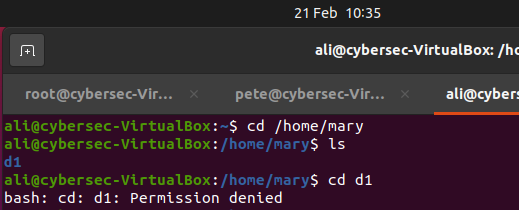
\includegraphics[width=.9\linewidth]{lab1/6}
    \caption{Encoding the plaintext with AES-256-cbc using the key "secretkey".}
    \label{fig:AESEncrypt}
\end{figure}

In this command, the -des flag is instead replaced by -aes-256-cbc, indicating the cipher to use, and the optional
-salt flag was added, which salts the text to provide different ciphertext.
Salting is the process of adding random data to the end of the text prior to encoding it, which will change
the resulting ciphertext, making it harder to decrypt and increasing the strength of the encryption.

\pagebreak

\section{Asymmetric encryption}\label{sec:asymmEncryption}
Asymmetric cryptography is the practice of using two keys when transmitting data: a public key used to encrypt
data, and a private key used to decrypt it.
For example: John is sending Alex an encrypted message.
The message is encrypted using Alex's public key and sent to Alex.
When Alex receives the message, it is decrypted using Alex's private key.
Alex can prove that John sent this message because of the digital signature attached, which is generated
from John's private key, and then verified using his public key.
John does not ever know what Alex's private key is, nor does Alex know John's private key.

Data transferred this way has a digital signature attached, which allows for non-repudiation, as it cannot
be denied that the data originated from the device with said signature.
The signature is validated using the sender's private key. \newline


\subsection{Generating an RSA private key}\label{subsec:rsa-private-key}
OpenSSL can be used to generate these keys by using the "openssl genrsa" command.

\begin{figure}[H]
    \centering
    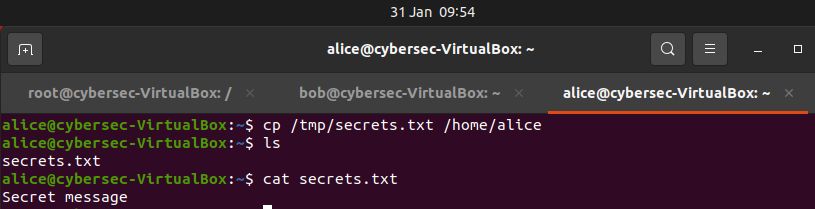
\includegraphics[width=.9\linewidth]{lab1/7}
    \caption{Generating a 2048-bit private key using genrsa.}
    \label{fig:genrsa}
\end{figure}

This works to generate a private key, but this command merely outputs it to the console, and does not actually
store it anywhere on the system.

\pagebreak

\subsection{Storing DES3 \& passphrase encrypted RSA keys in a file}\label{subsec:storing-keys-in-file}
The key generated can then be encrypted using an encryption algorithm, which would be DES3 for this example,
and a passphrase.
Upon doing this, the key can be stored into a .pem file, also known as a Privacy Enhanced Mail file, which is
a file format 'to provide the creation and validation of digital signatures, and in addition the
encryption and decryption of signed data, based on asymmetric and symmetric cryptography.'
~\autocite[p. 1894]{PEMFormat}

In this example, a 1024-bit key is created using DES3 and the passphrase
\footnote{The passphrase is not visible when typed, and therefore does not show in the image.} "secretkey".

\begin{figure}[H]
    \centering
    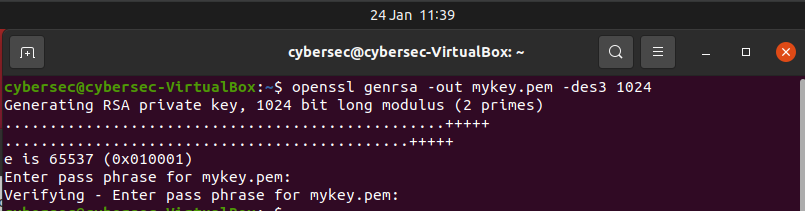
\includegraphics[width=.8\linewidth]{lab1/8}
    \caption{Generating and storing a 1024-bit private key using genrsa, DES3 and the passphrase "secretkey".}
    \label{fig:DES3Key}
\end{figure}

To break down this command:
\begin{itemize}
    \item genrsa - Generate an RSA private key.
    \item -out mykey.pem - Save the generated key to the file "mykey.pem" in the current directory.
    \item -des3 - Using the DES3 encryption method.
    \item 1024 - The key will be 1024 bits.\newline
\end{itemize}


We can then view this key by entering the command "more mykey.pem".

\begin{figure}[H]
    \centering
    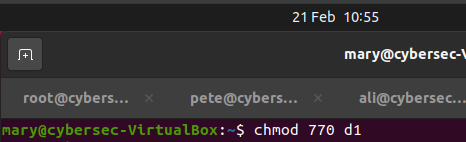
\includegraphics[width=.8\linewidth]{lab1/9}
    \caption{The key stored in mykey.pem.}
    \label{fig:mykey}
\end{figure}

\subsection{Getting a public key from the private key}\label{subsec:PubFromPriv}
The private key stored into "mykey.pem" by the previous command can be accessed again to generate
a public key, which would be used when data is encrypted.
To do so, the passphrase we set earlier (secretkey) must be entered.

\begin{figure}[H]
    \centering
    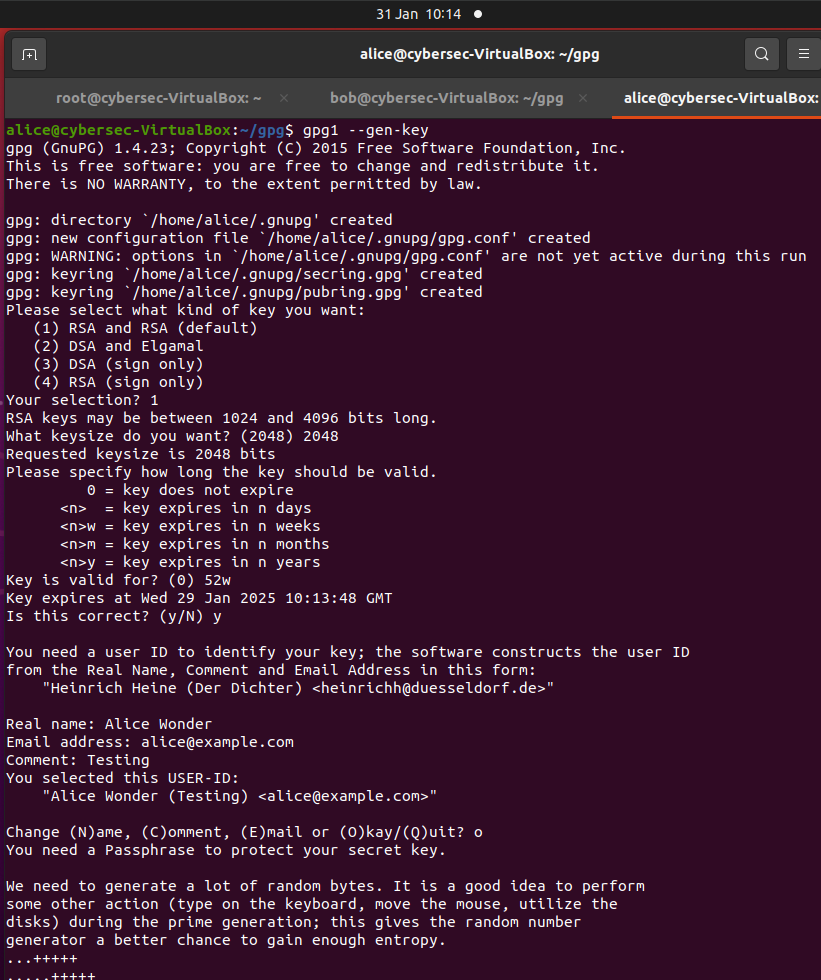
\includegraphics[width=.9\linewidth]{lab1/10}
    \caption{The public key generated from mykey.pem.}
    \label{fig:pubKey}
\end{figure}

Breaking down this command, "-in mykey.pem" uses mykey.pem as the input for the command, and
"-pubout" outputs the public key generated from the private key.
However, this command only outputs said key to the console, so an altered version is necessary to save
the key to a file.

\begin{figure}[H]
    \centering
    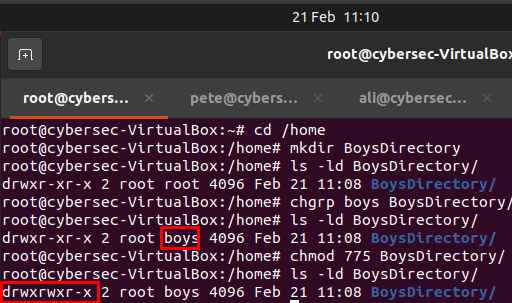
\includegraphics[width=.9\linewidth]{lab1/11}
    \caption{Storing the public key in a file.}
    \label{fig:pubKeyFile}
\end{figure}

The additional argument "-out public" is set in this command, meaning the public key will be written to
a file called "public".
This file can then be read using the cat command, revealing the public key seen in Figure \ref{fig:pubKey}.

\pagebreak

\subsection{Obtaining a message/file digest}\label{subsec:hashDigest}
When data is transmitted, it could become corrupted or potentially even intercepted and modified before it
reaches its intended recipient.
To mitigate the risks from this, files can have "digests", which are the result of hashing their contents.
If the file is modified whatsoever, even by a single byte, the digest would be different, meaning the file
has been corrupted or tampered with.
These are also the basis of digital signatures; by encrypting a digest with your private key, you cannot
deny that you were the source of the file.\newline

OpenSSL can generate digests using its "dgst" command.
\begin{figure}[H]
    \centering
    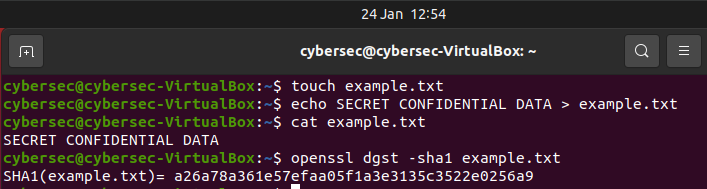
\includegraphics[width=.9\linewidth]{lab1/12}
    \caption{Creating a file, then getting the SHA1 digest of it.}
    \label{fig:digest}
\end{figure}

This can also be verified by using a non-OpenSSL command, sha1sum, which returns the same digest as the
OpenSSL dgst.

\begin{figure}[H]
    \centering
    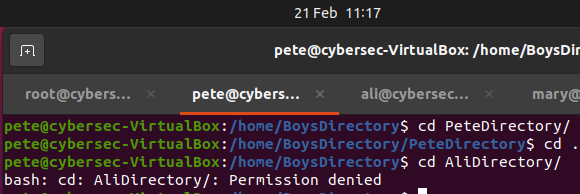
\includegraphics[width=.9\linewidth]{lab1/13}
    \caption{Verifying the digest.}
    \label{fig:digestVerify}
\end{figure}

\pagebreak

\subsection{Signing a digest}\label{subsec:SignDigest}
Non-repudiation is an important topic in cybersecurity - verifying the original sender of a file is an
imperative task in the event of any issues that may arise such as malware being appended to the file,
in either the prosecution or defense of the alleged sender.
Signing a message digest using your private key definitively proves the device that data was sent from,
meaning that it cannot be denied that the file was sent, nor who it was sent by.

The previously used "example.txt" can again be used here to generate a digest encrypted using the "mykey.pem"
private key established earlier, which signs the digest.

\begin{figure}[H]
    \centering
    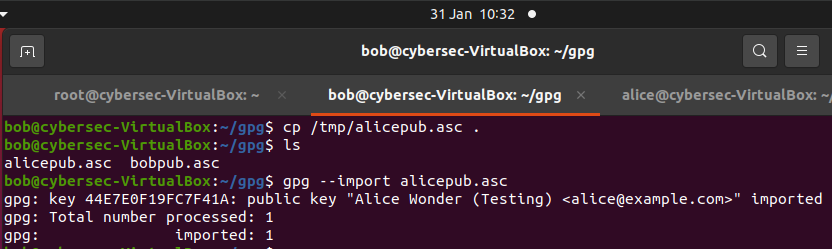
\includegraphics[width=.9\linewidth]{lab1/14}
    \caption{Writing a signed digest to a file.}
    \label{fig:writeDigest}
\end{figure}

Note that when we try to read this file, it is completely illegible, as it is not in a compatible format.
To counteract this, it can be converted to Base64 using OpenSSL's "enc" command, passing the generated file
as the argument.

\begin{figure}[H]
    \centering
    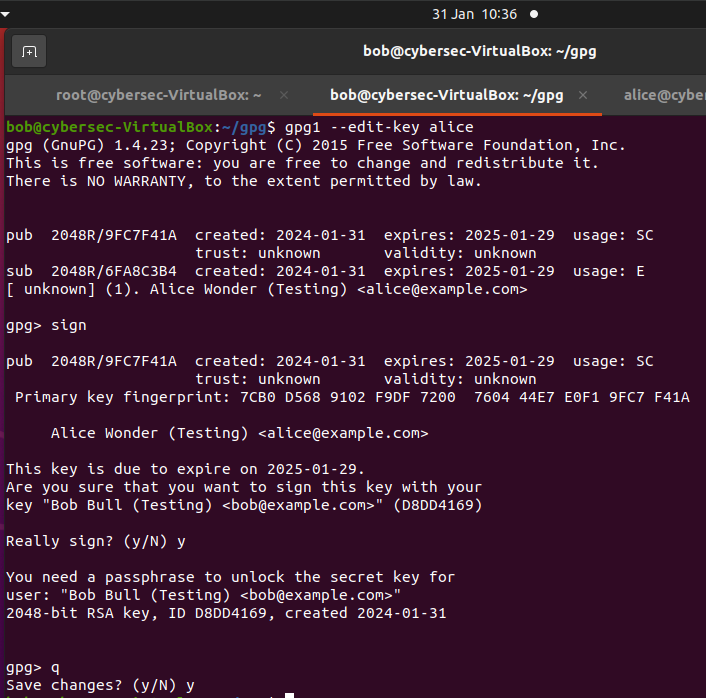
\includegraphics[width=.9\linewidth]{lab1/15}
    \caption{Encoding the signed digest to Base64.}
    \label{fig:base64Digest}
\end{figure}

This doesn't have any use other than allowing us to see the key in a Base64 format - the key functions even
if it can't be conventionally read. \newline

Now that we have the signed digest, it can be verified using the public key, which confirms the authenticity
of the data in example.txt.

\begin{figure}[H]
    \centering
    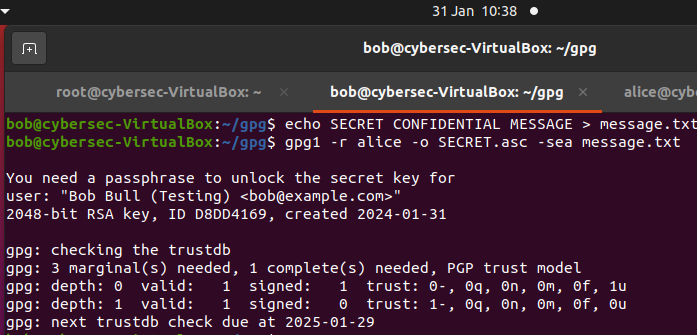
\includegraphics[width=.9\linewidth]{lab1/16}
    \caption{Verifying the signature of example.txt.}
    \label{fig:signatureVerify}
\end{figure}

This returns "Verified OK" as intended, as the file has not been modified.
If the file does get modified through either corruption or a threat actor, the digest would not be the same,
which can be verified by modifying the file ourselves and then verifying the digest of the file once again.

\begin{figure}[H]
    \centering
    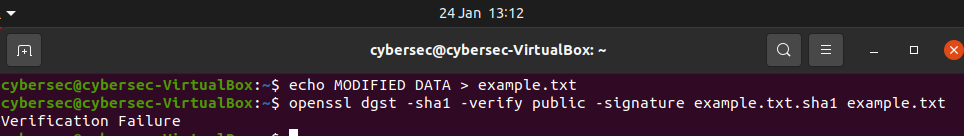
\includegraphics[width=.9\linewidth]{lab1/17}
    \caption{Failing to verify the signature of example.txt, as it has been modified.}
    \label{fig:signatureVerifyFail}
\end{figure}

This returns "Verification Failure", as the digest would now be different due to example.txt now containing
different data than it did when the SHA1 digest was created.




